\scanpage{88}

\diagram{%
\begin{tikzcd}[ampersand replacement=\&,column sep=0pt,row sep=0pt]
|[inner sep=0pt]| \vcenter{\hbox{%
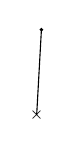
\begin{tikzpicture}[x=0.06cm,y=-0.06cm,line cap=round,line join=round,line width=.4pt]
\draw (1,0) -- (0,18);
\fill (1,0) circle[radius=0.025cm];
\node[inner sep=.55pt,anchor=center,font=\tiny] at (0,18) {$\times$};
\end{tikzpicture}%
}}
\end{tikzcd}%
}

\diagram{%
\begin{tikzcd}[ampersand replacement=\&,column sep=0pt,row sep=0pt]
|[inner sep=0pt]| \vcenter{\hbox{%
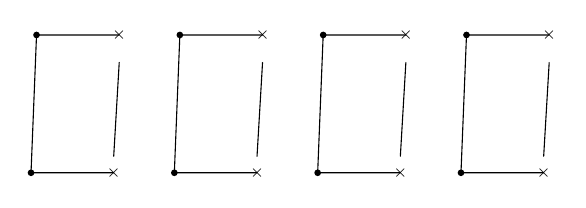
\begin{tikzpicture}[x=0.07cm,y=-0.07cm,line cap=round,line join=round,line width=.4pt]
\draw (15,0) -- (0,0) -- (-1,25) -- (14,25);
\draw (15,5) -- (14,22);
\fill (0,0) circle[radius=0.042499999999999996cm];
\fill (-1,25) circle[radius=0.042499999999999996cm];
\node[inner sep=.55pt,anchor=center,font=\tiny] at (15,0) {$\times$};
\node[inner sep=.55pt,anchor=center,font=\tiny] at (14,25) {$\times$};
\draw (41,0) -- (26,0) -- (25,25) -- (40,25);
\draw (41,5) -- (40,22);
\fill (26,0) circle[radius=0.042499999999999996cm];
\fill (25,25) circle[radius=0.042499999999999996cm];
\node[inner sep=.55pt,anchor=center,font=\tiny] at (41,0) {$\times$};
\node[inner sep=.55pt,anchor=center,font=\tiny] at (40,25) {$\times$};
\draw (67,0) -- (52,0) -- (51,25) -- (66,25);
\draw (67,5) -- (66,22);
\fill (52,0) circle[radius=0.042499999999999996cm];
\fill (51,25) circle[radius=0.042499999999999996cm];
\node[inner sep=.55pt,anchor=center,font=\tiny] at (67,0) {$\times$};
\node[inner sep=.55pt,anchor=center,font=\tiny] at (66,25) {$\times$};
\draw (93,0) -- (78,0) -- (77,25) -- (92,25);
\draw (93,5) -- (92,22);
\fill (78,0) circle[radius=0.042499999999999996cm];
\fill (77,25) circle[radius=0.042499999999999996cm];
\node[inner sep=.55pt,anchor=center,font=\tiny] at (93,0) {$\times$};
\node[inner sep=.55pt,anchor=center,font=\tiny] at (92,25) {$\times$};
\end{tikzpicture}%
}}
\end{tikzcd}%
}

\diagram{%
\begin{tikzcd}[ampersand replacement=\&,column sep=0pt,row sep=0pt]
|[inner sep=0pt]| \vcenter{\hbox{%
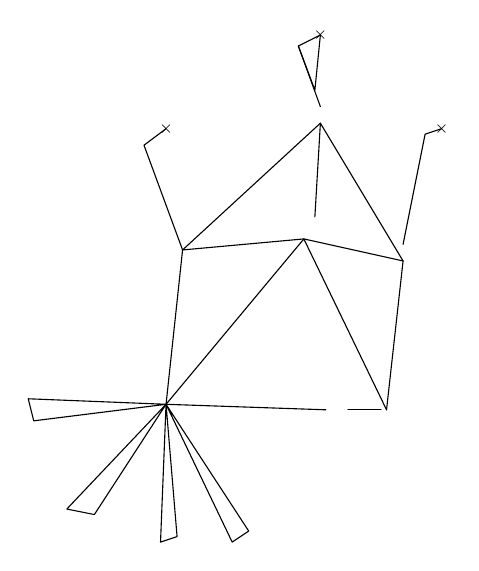
\begin{tikzpicture}[x=0.07cm,y=-0.07cm,line cap=round,line join=round,line width=.4pt]
\draw (25,67) -- (28,39) -- (53,16) -- (68,41) -- (65,68);
\draw (25,67) -- (50,37) -- (65,68);
\draw (28,39) -- (50,37) -- (68,41);
\draw (53,16) -- (52,33);
\draw (25,67) -- (54,68);
\draw (58,68) -- (64,68);
\draw (25,67) -- (0,66) -- (1,70) -- cycle;
\draw (25,67) -- (7,86) -- (12,87) -- cycle;
\draw (25,67) -- (24,92) -- (27,91) -- cycle;
\draw (25,67) -- (37,92) -- (40,90) -- cycle;
\draw (28,39) -- (21,20) -- (25,17);
\node[inner sep=.55pt,anchor=center,font=\tiny] at (25,17) {$\times$};
\draw (53,13) -- (49,2) -- (53,0);
\node[inner sep=.55pt,anchor=center,font=\tiny] at (53,0) {$\times$};
\draw (68,38) -- (72,18) -- (75,17);
\node[inner sep=.55pt,anchor=center,font=\tiny] at (75,17) {$\times$};
\draw (49,2) -- (52,10) -- (53,0);
\end{tikzpicture}%
}}
\end{tikzcd}%
}

\diagram{%
\begin{tikzcd}[ampersand replacement=\&,column sep=0pt,row sep=0pt]
|[inner sep=0pt]| \vcenter{\hbox{%
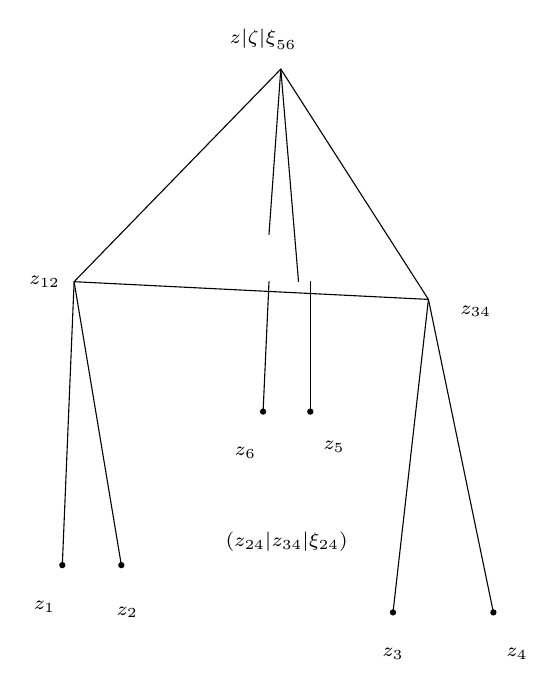
\begin{tikzpicture}[x=0.075cm,y=-0.075cm,line cap=round,line join=round,line width=.4pt]
\draw (15,36) -- (50,0) -- (75,39) -- cycle;
\draw (50,0) -- (48,28);
\draw (50,0) -- (53,36);
\draw (15,36) -- (13,84);
\draw (15,36) -- (23,84);
\fill (13,84) circle[radius=0.04cm];
\fill (23,84) circle[radius=0.04cm];
\draw (48,36) -- (47,58);
\draw (55,36) -- (55,58);
\fill (47,58) circle[radius=0.04cm];
\fill (55,58) circle[radius=0.04cm];
\draw (75,39) -- (69,92);
\draw (75,39) -- (86,92);
\fill (69,92) circle[radius=0.04cm];
\fill (86,92) circle[radius=0.04cm];
\node[inner sep=.55pt,anchor=center,font=\scriptsize] at (47,-5) {$\unsure{z|\zeta|\xi}_{56}$};
\node[inner sep=.55pt,anchor=center,font=\scriptsize] at (10,36) {$z_{12}$};
\node[inner sep=.55pt,anchor=center,font=\scriptsize] at (83,41) {$z_{34}$};
\node[inner sep=.55pt,anchor=center,font=\scriptsize] at (10,91) {$z_1$};
\node[inner sep=.55pt,anchor=center,font=\scriptsize] at (24,92) {$z_2$};
\node[inner sep=.55pt,anchor=center,font=\scriptsize] at (44,65) {$z_6$};
\node[inner sep=.55pt,anchor=center,font=\scriptsize] at (59,64) {$z_5$};
\node[inner sep=.55pt,anchor=center,font=\scriptsize] at (69,99) {$z_3$};
\node[inner sep=.55pt,anchor=center,font=\scriptsize] at (90,99) {$z_4$};
\node[inner sep=.55pt,anchor=center,font=\scriptsize] at (51,80) {$(\unsure{z_{24}|z_{34}|\xi_{24}})$};
\end{tikzpicture}%
}}
\end{tikzcd}%
}

\unsure{bicarroussel|bicaroussel|bicarrousel} épinglé

\unsure{autom} du bicarroussel d’ordre $48=2^4\cdot3$

\[
\begin{aligned}
\text{nb de \unsure{bicarousels|bicarrés|bicarrousels}} &\quad 2^3\,3^3\,5\\
&=6^3\cdot5=1080\\
&=\\
&=\underbrace{72}_{\text{\unsure{bases|racines}}}\ \underbrace{15}_{\substack{\text{nb de partitions}\\\text{d’un ens. à 6}\\\text{él. en parties}\\\text{à 2 él.}}}
\end{aligned}
\]

\diagram{%
\begin{tikzcd}[ampersand replacement=\&,column sep=0pt,row sep=0pt]
|[inner sep=0pt]| \vcenter{\hbox{%
\begin{tikzpicture}[x=0.076cm,y=-0.076cm,line cap=round,line join=round,line width=.4pt]
\draw (10,25) -- (0,59);
\draw (10,25) -- (4,71);
\draw (10,25) -- (11,60);
\draw (37,0) -- (29,28);
\draw (37,0) -- (37,37);
\draw (37,0) -- (46,35);
\draw (57,28) -- (49,68);
\draw (57,28) -- (57,78);
\draw (57,28) -- (66,68);
\draw (0,59) -- (4,62) -- (8,60) -- (11,61);
\node[inner sep=.55pt,anchor=center,font=\scriptsize] at (32,-10) {$z_{46}$};
\node[inner sep=.55pt,anchor=center,font=\scriptsize] at (108,-9) {$\deleted{\unsure{z_{36}}}\ z_{62}$};
\end{tikzpicture}%
}}
\end{tikzcd}%
}

\diagram{%
\begin{tikzcd}[ampersand replacement=\&,column sep=0pt,row sep=0pt]
|[inner sep=0pt]| \vcenter{\hbox{%
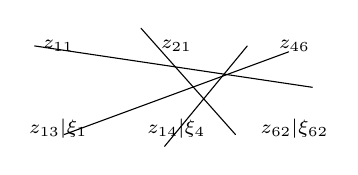
\begin{tikzpicture}[x=0.075cm,y=-0.075cm,line cap=round,line join=round,line width=.4pt]
\node[inner sep=.55pt,anchor=center,font=\scriptsize] at (0,0) {$\deleted{\unsure{z_{11}}}$};
\node[inner sep=.55pt,anchor=center,font=\scriptsize] at (20,0) {$\deleted{\unsure{z_{21}}}$};
\node[inner sep=.55pt,anchor=center,font=\scriptsize] at (40,0) {$\deleted{\unsure{z_{46}}}$};
\node[inner sep=.55pt,anchor=center,font=\scriptsize] at (0,14) {$\deleted{\unsure{z_{13}|\xi_1}}$};
\node[inner sep=.55pt,anchor=center,font=\scriptsize] at (20,14) {$\deleted{\unsure{z_{14}|\xi_4}}$};
\node[inner sep=.55pt,anchor=center,font=\scriptsize] at (40,14) {$\deleted{\unsure{z_{62}|\xi_{62}}}$};
\draw (-4,0) -- (43,7);
\draw (1,15) -- (39,1);
\draw (14,-3) -- (30,15);
\draw (18,17) -- (32,0);
\end{tikzpicture}%
}}
\end{tikzcd}%
}

\[
\begin{aligned}
&\frac{6!}{2!\,2!\,2!}\quad\cdot\binom62\binom42\frac1{3!}\\
&\qquad =\frac{15\cdot6}{6}\ =15
\end{aligned}
\]

% archive sheet number: 87
